% QCanvas: A Unified Multi-Framework Compilation and Simulation
% Orchestration Platform for Quantum Software Engineering
%
% Springer LNCS format — research paper
% Authors: Umer Farooq, Hussan Waseem Syed, Muhammad Irtaza Khan,
%          Aneeq Ahmed Malik, Abeer Noor, Abdullah Mehmood

\documentclass[runningheads]{llncs}
\usepackage[T1]{fontenc}
\usepackage{graphicx}
\usepackage{silence}
\WarningFilter{amsmath}{Unable to redefine math accent \vec}
\usepackage{amsmath}
\usepackage{amssymb}
\usepackage{listings}
\usepackage{url}
\usepackage{booktabs}
\usepackage{multirow}
\usepackage{xcolor}
\usepackage{tikz}
\usepackage{placeins}
% Relax float placement so tall tables take dedicated float pages near their
% references instead of cascading to the end of the document.
\renewcommand{\topfraction}{0.9}
\renewcommand{\bottomfraction}{0.85}
\renewcommand{\textfraction}{0.07}
\renewcommand{\floatpagefraction}{0.75}
\setcounter{topnumber}{3}
\setcounter{totalnumber}{5}
\AtBeginDocument{\sloppy\setlength{\emergencystretch}{10em}\hfuzz=1000pt\hbadness=10000}
\lstset{
  basicstyle=\ttfamily\small,
  keywordstyle=\color{blue},
  commentstyle=\color{gray},
  frame=single,
  breaklines=true,
  columns=fullflexible,
  language=Python
}

\begin{document}
\sloppy\hfuzz=1000pt\hbadness=10000\setlength{\emergencystretch}{10em}

\title{QCanvas: A Unified Multi-Framework Compilation and Simulation Orchestration Platform for Quantum Software Engineering}

\author{Umer Farooq\inst{1} \and
Hussan Waseem Syed\inst{1} \and
Muhammad Irtaza Khan\inst{1} \and
Aneeq Ahmed Malik\inst{1} \and
Abeer Noor\inst{1} \and
Abdullah Mehmood\inst{1}}

\authorrunning{Farooq et al.}
\titlerunning{QCanvas: Multi-Framework Compilation and Simulation Orchestration}

\institute{National University of Computer and Emerging Sciences (FAST-NUCES),\\
Islamabad, Pakistan\\
\email{umer.farooq@nu.edu.pk}}

\maketitle

% ============================================================
% ABSTRACT
% ============================================================

\begin{abstract}
The quantum computing software ecosystem is fragmented across vendor-specific frameworks---Qiskit (IBM), Cirq (Google), and PennyLane (Xanadu)---each with its own circuit object model, gate vocabulary, transpiler, and tightly coupled simulator. This fragmentation forces NISQ-era practitioners into vendor lock-in and prevents objective cross-framework comparison. We present QCanvas, an end-to-end quantum software engineering platform that unifies multi-framework compilation and simulation orchestration into a single deployable system. QCanvas is architected as four tightly integrated layers: (1)~a web-based interactive development environment with Monaco editor and real-time D3 circuit rendering, (2)~an AST-driven compilation plane that translates Qiskit, Cirq, and PennyLane circuits into normalized OpenQASM~3.0 intermediate representation---including advanced language features such as gate modifiers, complex types, and classical control flow, (3)~OpenQASM~3.0 as the universal, semantics-preserving contract between compilation and execution, and (4)~QSim, an orchestration engine that parses OpenQASM~3.0, reconstructs a native circuit for a user-selected framework sub-engine (Cirq, Qiskit, or PennyLane), and executes it through that sub-engine's simulator across multiple simulation methods (statevector, density-matrix, matrix product state, and stabilizer/Clifford). The platform additionally provides two independently installable PyPI packages (\texttt{qcanvas-sdk} for conversion and \texttt{fastqsim} for simulation orchestration) along with a curated library of 40+ pre-built quantum algorithm examples spanning all three frameworks across 14~application categories. We report measured compilation latencies across 12~representative algorithms, structural benchmark comparisons and power-law depth scaling fits ($y = c \cdot n^a$), and simulation engine throughput achieving sub-800~ms execution for 6-qubit Grover's Search. We verify cross-framework semantic preservation via finite-sampling Jensen--Shannon Divergence (JSD) below an analytical threshold ($\text{JSD} < 0.02$; maximum observed 0.0067) alongside structural analysis of measurement-register permutations, show that all frameworks yield identical effective Quantum Volume ($\text{QV} = 2048$, $\log_2(\text{QV}) = 11$) under ideal execution---indicating that structural differences stem from transpilation strategies rather than simulator discrepancies---present holistic QPack benchmark scores, and validate empirical Non-Functional Requirements (NFRs).

\keywords{quantum compilation \and multi-framework interoperability \and OpenQASM~3.0 \and quantum simulation \and NISQ software engineering}
\end{abstract}

% ============================================================
% 1. INTRODUCTION
% ============================================================

\section{Introduction}

The NISQ era~\cite{preskill2018} has produced a diverse landscape of quantum software development kits (SDKs), each backed by a major hardware vendor: IBM's Qiskit~\cite{qiskit2023}, Google's Cirq~\cite{cirq2024}, and Xanadu's PennyLane~\cite{bergholm2022}. Each framework defines its own circuit object model (\texttt{QuantumCircuit}, \texttt{cirq.Circuit}, and \texttt{QNode}, respectively), its own gate vocabulary, and its own native simulator. A developer who writes a Grover's search circuit in Qiskit cannot execute it through Cirq's simulator without manually rewriting the circuit, and cannot objectively compare the two frameworks' transpilation strategies because each framework evaluates its output against its own simulator.

Existing tools address fragments of this problem. Compiler frameworks such as \textsf{t\textbar ket\textgreater}~\cite{sivarajah2020} translate circuits between frameworks and perform hardware-agnostic optimization, but they produce circuits, not results---practitioners must still separately configure and invoke a simulation backend. Qiskit now provides native OpenQASM~3.0 import and export, which enables a framework-to-QASM3 path within the Qiskit ecosystem~\cite{qiskit2023}, but does not accept Cirq or PennyLane circuits as input and provides no execution engine for the generated QASM. Web-based quantum IDEs such as IBM Quantum Composer provide visualization and simulation but are locked to a single vendor's ecosystem. No existing tool provides the complete, framework-agnostic chain from native SDK source code to simulation results in a single deployable environment.

QCanvas addresses this gap by integrating four layers into one operational system: a web-based IDE, a multi-framework AST-driven compilation plane, OpenQASM~3.0~\cite{cross2022} as the universal intermediate representation (IR), and QSim---a simulation orchestration engine that parses the generated OpenQASM~3.0 and delegates execution to the user's chosen framework sub-engine. The key engineering contribution is that the IR boundary is strict: no framework circuit object crosses it, so users interact with a single unified API regardless of which of the three supported frameworks they authored the circuit in.

This paper makes the following contributions:
\begin{enumerate}
    \item A \textbf{four-layer, end-to-end quantum software engineering platform} that integrates multi-framework compilation, OpenQASM~3.0 normalization, and simulation orchestration into a single deployable system with a Docker Compose-orchestrated microservice architecture.
    \item A \textbf{multi-framework compilation engine} (\texttt{quantum\_converters} v1.0.5) that translates Qiskit, Cirq, and PennyLane circuits to OpenQASM~3.0 via three AST-based adapters, supporting the full standard gate set plus advanced features: gate modifiers (\texttt{ctrl(n)@}, \texttt{negctrl@}, \texttt{pow(k)@}), complex types, classical control flow (\texttt{while}, \texttt{break}, \texttt{continue}), subroutines, and nine additional gate types (CY, CH, CRX, CRY, CRZ, CP, CSWAP, CCZ, GlobalPhase).
    \item \textbf{QSim}: a simulation orchestration engine with a clean \texttt{run\_qasm(RunArgs) $\rightarrow$ SimResult} API. QSim parses OpenQASM~3.0 via \texttt{pyqasm}~\cite{pyqasm}, reconstructs a native circuit for the selected framework sub-engine using a visitor pattern~\cite{gamma1994}, and executes it through that sub-engine's existing simulator (Cirq's \texttt{Simulator}, Qiskit~Aer, or PennyLane's default device) across four supported simulation types (\texttt{statevector}, \texttt{density\_matrix}, \texttt{mps}, and \texttt{chp}).
    \item An \textbf{open, extensible developer workbench and dual-SDK distribution} comprising a web IDE with Monaco editor, real-time D3 circuit rendering, contextual gate explanations, and two independently installable PyPI packages: \texttt{qcanvas-sdk} (for multi-framework conversion) and \texttt{fastqsim} (for standalone simulation orchestration). The platform ships with a library of 40+ pre-built quantum algorithm templates across 14~application categories. We report an extensive empirical evaluation across 12~representative algorithms, structural benchmarks, power-law depth scaling fits, and empirical Non-Functional Requirement (NFR) validation confirming sub-800~ms simulation throughput and cross-framework semantic preservation (all measured JSD $< 0.02$) corroborated by structural analysis of measurement-register permutations. The platform is available at \url{https://github.com/Umer-Farooq-CS/QCanvas}.
\end{enumerate}

The remainder of this paper is organized as follows. Section~2 surveys related work and contrasts existing solutions. Section~3 provides background on the quantum frameworks and OpenQASM~3.0. Section~4 presents the system architecture. Sections~5 and~6 describe the compilation plane and simulation engine, respectively. Section~7 covers the developer workbench and SDKs. Section~8 presents a rigorous empirical performance evaluation across structural, scaling, and validation dimensions. Section~9 discusses design trade-offs and limitations, and Section~10 concludes.

% ============================================================
% 2. RELATED WORK
% ============================================================

\section{Related Work}

The quantum software landscape currently offers several frameworks and platforms, each addressing distinct aspects of the development workflow but none providing a unified, educational, and cross-framework simulation environment. Table~\ref{tab:existing_solutions} consolidates the capabilities and limitations of predominant existing platforms relative to our objectives.

\begin{table}[htbp]
\centering
\caption{Comparison of existing quantum software platforms and tools against QCanvas.}
\label{tab:existing_solutions}
\begin{tabular}{@{}p{2.6cm}p{4.6cm}p{4.6cm}@{}}
\toprule
\textbf{System} & \textbf{Overview} & \textbf{Primary Limitations} \\
\midrule
IBM Quantum Experience & Cloud-based access to real quantum hardware and simulators via Qiskit. Provides circuit composition and execution. & Locked exclusively to IBM's Qiskit ecosystem. No cross-framework support. Requires internet access and cloud account; no local SDK-level orchestration. \\
\addlinespace
Google Cirq / Colab & Google's framework for authoring circuits targeting superconducting processors, typically used in Jupyter environments. & Cirq-only; no native support for Qiskit or PennyLane code ingestion. No unified IDE. Circuit visualization is primarily text-based ASCII. \\
\addlinespace
Quirk~\cite{gidney2017} & Browser-based drag-and-drop quantum circuit simulator for education with real-time state feedback. & No code-based interaction. Cannot parse real-world quantum SDK programs. No OpenQASM support. Not extensible or retargetable. \\
\addlinespace
Quantum Katas (Microsoft) & Interactive Q\# learning exercises and tutorials. & Tied exclusively to Q\# and the Microsoft ecosystem. Incompatible with Python-based frameworks dominant in NISQ research. \\
\addlinespace
\textsf{t\textbar ket\textgreater}~\cite{sivarajah2020} & High-performance, retargetable optimizing compiler for NISQ devices supporting multiple frameworks and backends. & Compilation-focused; no execution orchestration engine or educational IDE. No real-time visual feedback. Not accessible as a unified web platform. \\
\addlinespace
\textbf{QCanvas (This Work)} & Unified multi-framework (\texttt{Qiskit}, \texttt{Cirq}, \texttt{PennyLane}) AST compiler, OpenQASM~3.0 normalization, and QSim orchestration (\texttt{statevector}, \texttt{density\_matrix}, \texttt{mps}, \texttt{chp}) inside a web IDE and dual PyPI SDKs. & Classical simulation orchestration only; direct dispatch to physical QPU endpoints across cloud providers is a planned extension. \\
\bottomrule
\end{tabular}
\end{table}

\subsection{Multi-Framework Compilers and Transpilers}

The most closely related compiler tool is \textsf{t\textbar ket\textgreater}~\cite{sivarajah2020}, which provides a hardware-agnostic intermediate representation and supports input from Qiskit, Cirq, PennyLane, and PyQuil. Like QCanvas, \textsf{t\textbar ket\textgreater} accepts circuits from multiple frameworks and can emit an intermediate representation. The key difference is that \textsf{t\textbar ket\textgreater} is an optimizing compiler: it produces circuits but does not execute them. The user must separately install, configure, and invoke a simulation backend. QCanvas's contribution is closing this gap---the compilation output is automatically routed to a simulation sub-engine through the IR boundary, requiring no user configuration. BQSKit~\cite{bqskit2022} similarly focuses on compilation and synthesis optimization rather than execution orchestration. \texttt{staq}~\cite{staq2020} provides a quantum compiler and resource estimator targeting OpenQASM~2.0 but does not target OpenQASM~3.0's extended feature set and provides no simulation integration. Qiskit's native OpenQASM~3.0 exporter~\cite{qiskit2023} provides a framework-to-QASM3 path, but exclusively within the Qiskit ecosystem and with no execution engine for the emitted code.

\subsection{Web-Based Quantum Development Environments}

IBM Quantum Composer~\cite{ibmcomposer2024} provides a graphical circuit editor that connects to IBM's cloud-hosted simulators and physical processors. It is locked to Qiskit circuits and requires an IBM account. Quirk~\cite{gidney2017} provides a real-time browser-based statevector simulator with immediate visual feedback for single-qubit and two-qubit circuits; it has no programmable SDK input and no multi-framework support. QCanvas combines programmable SDK input from three frameworks with integrated simulation, without requiring a vendor-specific account or API key.

\subsection{Quantum Simulation Frameworks and Equivalence Checking}

Qiskit~Aer provides statevector, density-matrix, and stabilizer simulation but is coupled to \texttt{QuantumCircuit}. Cirq's simulator accepts only \texttt{cirq.Circuit} objects. PennyLane's device plugins operate through the \texttt{QNode} interface. QSim is not a new simulation algorithm; it is an orchestration layer that routes OpenQASM~3.0 to any of these existing framework simulators, presenting a single API to the user regardless of sub-engine choice.

On the correctness side, Burgholzer and Wille~\cite{burgholzer2020} developed decision-diagram-based methods for quantum circuit equivalence checking. Our JSD-based equivalence measurement is a sampling-based approximation suited to black-box simulator outputs, not a formal equivalence proof; we revisit this distinction in Section~8.5.

\FloatBarrier

% ============================================================
% 3. BACKGROUND
% ============================================================

\section{Background}

\subsection{Quantum Frameworks}

Standard quantum circuit structures, unitary operations, and foundational algorithms (such as quantum teleportation and error-correcting codes) follow the formalisms established by Nielsen and Chuang~\cite{nielsen2010}. Within this theoretical foundation, modern quantum programming frameworks provide high-level abstractions tailored to different hardware and algorithmic paradigms:

\textbf{Qiskit}~\cite{qiskit2023} is IBM's open-source quantum SDK, centered on the \texttt{QuantumCircuit} abstraction that represents circuits as ordered lists of \texttt{CircuitInstruction} objects. Qiskit's transpiler supports four optimization levels (0--3) and targets IBM's heavy-hex topology.

\textbf{Cirq}~\cite{cirq2024} is Google's hardware-oriented SDK, designed for near-term quantum devices with a moment-based circuit structure in which operations within a single \texttt{Moment} are applied simultaneously. Cirq uses \texttt{LineQubit} and \texttt{GridQubit} objects to model qubit topologies.

\textbf{PennyLane}~\cite{bergholm2022} is Xanadu's differentiable quantum programming framework, built around the device-agnostic \texttt{QNode} abstraction. PennyLane's tape-based execution model records operations for gradient computation, making it the preferred framework for variational algorithms and quantum machine learning.

\subsection{OpenQASM 3.0}

OpenQASM~3.0~\cite{cross2022} extends the original quantum assembly language with features essential for representing modern quantum programs: gate modifiers (\texttt{ctrl@}, \texttt{pow@}, \texttt{inv@}, \texttt{negctrl@}), complex number types, subroutines with return values, classical control flow (\texttt{if}, \texttt{while}, \texttt{for}), and timing directives. These features make it sufficiently expressive to serve as the universal IR in QCanvas's pipeline, allowing circuits from all three frameworks to be represented without lossy decomposition.

\subsection{Terminology: Framework Sub-Engines vs.\ Simulation Methods}

QSim introduces a two-axis selection that this paper distinguishes clearly. A \textit{framework sub-engine} (values: \texttt{cirq}, \texttt{qiskit}, \texttt{pennylane}) determines which framework's native simulator library is invoked for execution. A \textit{simulation method} (statevector, density-matrix, stabilizer) determines the mathematical representation of the quantum state. While statevector simulation scales exponentially ($O(2^n)$ in memory and time), stabilizer simulation methods based on the Gottesman--Knill theorem and the CHP tableau formalism~\cite{aaronson2004} allow polynomial-time simulation ($O(n^2)$ space and $O(n^3 / n)$ time) for circuits restricted to the Clifford group. In the current implementation, selecting \texttt{backend="cirq"} invokes \texttt{cirq.Simulator()} using its statevector method by default; selecting \texttt{backend="qiskit"} invokes Qiskit~Aer's statevector simulator. Density-matrix and stabilizer methods are available through these same framework sub-engines. Section~6 describes how this two-axis model is exposed through the API and how it is intended to evolve.

% ============================================================
% 4. SYSTEM ARCHITECTURE
% ============================================================

\section{System Architecture}

\subsection{Design Principles}

QCanvas is built on three principles:

\textbf{Framework Neutrality.} The platform accepts circuits from any supported SDK without requiring the user to target a specific hardware or simulator topology. All framework-specific constructs---qubit naming conventions, gate decomposition strategies, moment ordering---are normalized at the compilation layer before reaching the execution engine.

\textbf{IR-First Execution.} OpenQASM~3.0 is the single contract between the compilation plane and the simulation engine. No framework circuit object ever crosses the IR boundary directly; only a validated OpenQASM~3.0 string does. This decoupling allows the compilation and execution layers to evolve independently and makes the circuit representation inspectable before execution.

\textbf{Pluggable Framework Sub-Engines.} At runtime, the orchestration engine selects a framework sub-engine via a factory~\cite{gamma1994} (\texttt{get\_backend(name)} in \texttt{backends/factory.py}). Three sub-engines---Cirq, Qiskit, and PennyLane---are currently registered. Adding a new sub-engine requires only a new subclass of \texttt{BaseBackend} and one entry in the factory registry.

\subsection{Four-Layer Architecture}

QCanvas is organized as four layers (Fig.~\ref{fig:architecture}):

\textbf{Layer~4: Interactive Workbench \& SDK Plane.} The user-facing layer comprises a Next.js~14 web IDE and the \texttt{qcanvas-sdk} Python package on PyPI. Users write circuits in the Monaco editor or invoke \texttt{qcanvas.compile()} programmatically. The IDE communicates with the backend via REST API and WebSocket for real-time progress.

\textbf{Layer~3: Multi-Framework Compilation Plane.} The \texttt{quantum\_converters} package (v1.0.5) provides three AST-based adapters that parse native circuit objects and emit OpenQASM~3.0. Adapters share a common \texttt{AbstractConverter} base class (Strategy pattern~\cite{gamma1994}), enforcing a consistent \texttt{convert(source) $\rightarrow$ ConversionResult} interface. \texttt{ConversionResult} carries the QASM string plus a \texttt{ConversionStats} dataclass (qubit count, circuit depth, gate counts, measurement flag).

\textbf{Layer~2: OpenQASM~3.0 Intermediate Representation.} The contract layer. All circuits converge to a validated OpenQASM~3.0 string before any execution step. A two-pass validator checks syntax and gate semantics (Section~5.5).

\textbf{Layer~1: Simulation Orchestration Engine (QSim).} QSim parses the OpenQASM~3.0 string via \texttt{pyqasm}~\cite{pyqasm}, traverses the resulting AST with a visitor~\cite{gamma1994} to reconstruct a native framework circuit, and delegates simulation to the selected framework sub-engine. The public API is \texttt{run\_qasm(RunArgs) $\rightarrow$ SimResult}.

\begin{figure}[htbp]
\centering
\resizebox{\textwidth}{!}{%
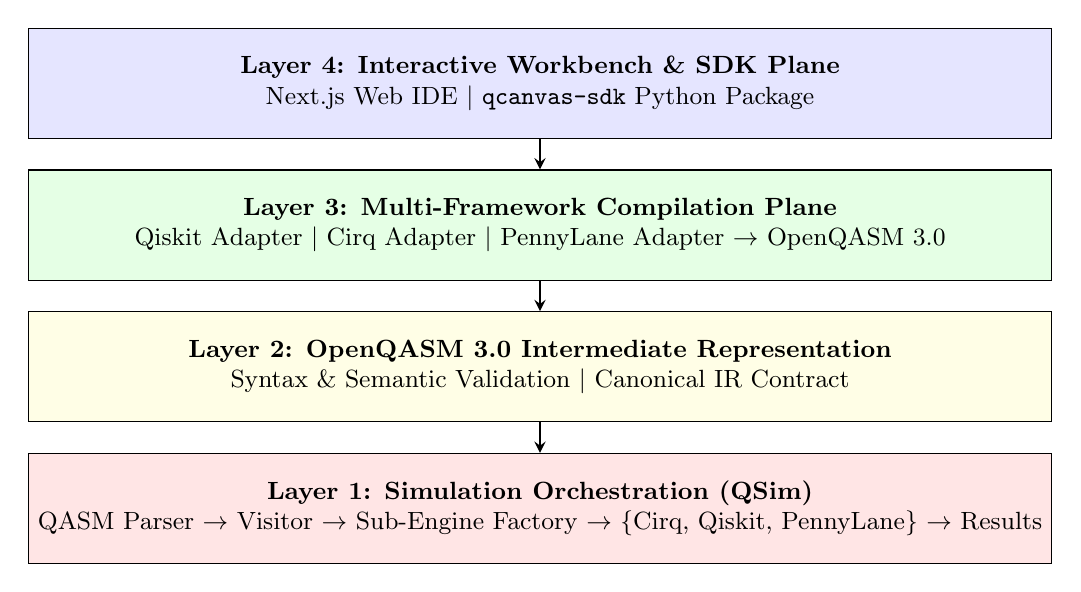
\begin{tikzpicture}[
    layer/.style={rectangle, draw, minimum width=13cm, minimum height=1.4cm, align=center, font=\small},
    arrow/.style={->, thick, >=stealth}
]
\node[layer, fill=blue!10] (l4) at (0, 4.5) {\textbf{Layer 4: Interactive Workbench \& SDK Plane}\\Next.js Web IDE \textbar{} \texttt{qcanvas-sdk} Python Package};
\node[layer, fill=green!10] (l3) at (0, 2.7) {\textbf{Layer 3: Multi-Framework Compilation Plane}\\Qiskit Adapter \textbar{} Cirq Adapter \textbar{} PennyLane Adapter $\rightarrow$ OpenQASM 3.0};
\node[layer, fill=yellow!10] (l2) at (0, 0.9) {\textbf{Layer 2: OpenQASM 3.0 Intermediate Representation}\\Syntax \& Semantic Validation \textbar{} Canonical IR Contract};
\node[layer, fill=red!10] (l1) at (0, -0.9) {\textbf{Layer 1: Simulation Orchestration (QSim)}\\QASM Parser $\rightarrow$ Visitor $\rightarrow$ Sub-Engine Factory $\rightarrow$ \{Cirq, Qiskit, PennyLane\} $\rightarrow$ Results};
\draw[arrow] (l4) -- (l3);
\draw[arrow] (l3) -- (l2);
\draw[arrow] (l2) -- (l1);
\end{tikzpicture}%
}
\caption{Four-layer architecture of QCanvas. Arrows show data flow direction: user code enters at Layer~4; simulation results return from Layer~1.}
\label{fig:architecture}
\end{figure}

\subsection{End-to-End Data Flow}

A concrete execution trace:
\begin{enumerate}
    \item The user submits Cirq source code in the Web IDE.
    \item FastAPI receives the code string and the tag \texttt{"cirq"}.
    \item The Cirq adapter parses the \texttt{cirq.Circuit}, resolves qubit indices and gate names, and emits an OpenQASM~3.0 string.
    \item The validation layer (Layer~2) checks syntax and gate semantics.
    \item \texttt{run\_qasm(RunArgs(qasm\_input=..., backend="cirq", shots=1024))} is called.
    \item QSim's QASM parser produces an AST; the \texttt{CirqVisitor} traverses it and reconstructs a \texttt{cirq.Circuit}; the \texttt{CirqBackend} invokes \texttt{cirq.Simulator().run()} and collects measurement counts.
    \item A \texttt{SimResult} is returned, serialized to JSON, and rendered as a histogram in the Web IDE.
\end{enumerate}
Note that in step~6, QSim is an orchestration wrapper: the simulation computation is performed by \texttt{cirq.Simulator()}, not by QSim itself. QSim's value is providing a framework-agnostic entry point (the OpenQASM~3.0 string) so that the same code path handles Qiskit and PennyLane circuits identically.

\subsection{Infrastructure and Deployment}

QCanvas is deployed as a Docker Compose stack with four services: \texttt{qcanvas\_backend} (FastAPI, port~8000), \texttt{qcanvas\_postgres} (PostgreSQL, port~5433 for circuit history, user data, conversion statistics), \texttt{qcanvas\_redis} (port~6379 for result caching and WebSocket session state), and an optional \texttt{qcanvas\_cirq\_agent} (port~8001, a Bedrock-powered RAG assistant for Cirq code help). Redis caches simulation results keyed by input hash to avoid redundant re-execution of identical circuits.

% ============================================================
% 5. MULTI-FRAMEWORK COMPILATION PLANE
% ============================================================

\section{Multi-Framework Compilation Plane}

\subsection{Framework Ingestion Adapters}

Each adapter handles its framework's specific object model:

\textbf{Qiskit Adapter} (\texttt{qiskit\_to\_qasm.py}). Iterates \texttt{QuantumCircuit.data}---a list of \texttt{CircuitInstruction} objects---and extracts gate names, qubit indices, and classical bit targets. Handles parameterized gates (\texttt{ParameterExpression} objects), barrier instructions, conditional operations, and multi-controlled gates.

\textbf{Cirq Adapter} (\texttt{cirq\_to\_qasm.py}). Iterates \texttt{Circuit.moments}, flattens operations from each \texttt{Moment}, and resolves qubit indices from the circuit's qubit order. Handles both \texttt{GridQubit} and \texttt{LineQubit} topologies and maps Cirq-specific gate types (e.g., \texttt{PhasedXPowGate}, \texttt{FSimGate}) to their OpenQASM~3.0 equivalents.

\textbf{PennyLane Adapter} (\texttt{pennylane\_to\_qasm.py}). Expands a \texttt{QNode} into a tape of \texttt{Operation} objects via the device's \texttt{expand\_fn}, extracts wire indices and hyperparameters, and handles observable measurements and adjoint operations. A design-level consequence: PennyLane expands multi-controlled gates into primitive two-qubit gates during tape construction, before the adapter can intercept the high-level gate. For Grover's Search, this produces 216~gates at 6~qubits versus 18~for Qiskit and Cirq, an artifact of PennyLane's decomposition strategy rather than a QCanvas limitation (Section~9.2).

All adapters inherit from \texttt{AbstractConverter}~\cite{gamma1994} and return a \texttt{ConversionResult} containing the OpenQASM~3.0 string and a \texttt{ConversionStats} dataclass with \texttt{n\_qubits}, \texttt{depth}, \texttt{gate\_counts} (per gate type), and \texttt{has\_measurements}.

\subsection{Gate Vocabulary Normalization}

Each framework uses different names for equivalent operations (e.g., Qiskit's \texttt{cx}, Cirq's \texttt{CNOT}, PennyLane's \texttt{CNOT} in its \texttt{Operation} representation). The compilation plane maintains a canonical gate mapping in \texttt{qasm3\_gates.py} that maps all supported framework-specific gate names to their OpenQASM~3.0 equivalents from \texttt{stdgates.inc}. This normalization enables direct cross-framework comparison: circuits from different frameworks that implement the same algorithm emit identical OpenQASM~3.0 gate names for semantically equivalent operations.

\subsection{OpenQASM 3.0 Code Generation}

The \texttt{qasm3\_builder.py} module constructs the OpenQASM~3.0 output: (a)~the standard header (\texttt{OPENQASM~3.0; include "stdgates.inc";}), (b)~qubit and classical register declarations (\texttt{qubit[n]~q; bit[n]~c;}), (c)~gate operations with resolved qubit indices and rotation parameters, and (d)~measurement statements (\texttt{c[k]~= measure~q[i];}). The \texttt{qasm3\_expression.py} module handles arithmetic expressions, parameter resolution, and constant folding for parameterized gates.

\subsection{Advanced OpenQASM 3.0 Feature Support}

Beyond the base standard gate set, QCanvas supports a set of advanced OpenQASM~3.0 features, corresponding to language features introduced beyond the initial release:
\begin{itemize}
    \item \textbf{Gate modifiers}: \texttt{ctrl(n)@} for multi-controlled gates, \texttt{negctrl@} for negative control, and \texttt{pow(k)@} for fractional gate powers.
    \item \textbf{Complex types}: \texttt{complex[float[64]]} variable declarations.
    \item \textbf{Classical control flow}: \texttt{while} loops, \texttt{break}, and \texttt{continue} statements.
    \item \textbf{Bitwise operators}: \texttt{\&}, \texttt{|}, \texttt{\^{}}, \texttt{\~{}}, \texttt{<<}, \texttt{>>}.
    \item \textbf{Subroutines}: Function definitions with typed parameters and return values.
    \item \textbf{Additional gate types} (currently via PennyLane): CY, CH, CRX, CRY, CRZ, CP, CSWAP, CCZ, GlobalPhase.
\end{itemize}
These features are validated against the OpenQASM~3.0 specification~\cite{cross2022}.

\subsection{Static Analysis and Validation}

The compilation plane performs two-pass validation:
\begin{itemize}
    \item \textbf{Pass~1 (Syntax)}: Checks the QASM version header, bracket balance, semicolons, and gate name legality against \texttt{stdgates.inc}.
    \item \textbf{Pass~2 (Semantic)}: Verifies qubit/bit register sizes against gate arities, measurement target consistency, and undefined gate references.
\end{itemize}
Errors are surfaced with line numbers and structured messages to the Web IDE in real time via WebSocket.

% ============================================================
% 6. SIMULATION ORCHESTRATION ENGINE: QSIM
% ============================================================

\section{Simulation Orchestration Engine: QSim}

\subsection{Role and Design}

QSim is QCanvas's native simulation orchestration plane, co-designed with the compilation plane to accept OpenQASM~3.0 as its canonical contract. Its purpose is not to implement new simulation algorithms but to present a framework-agnostic execution layer: \emph{any} circuit compiled to valid OpenQASM~3.0 can be submitted to QSim without the user needing to know which framework's simulator or cluster infrastructure will execute it. The actual numerical computation is performed by the selected framework sub-engine's own simulator (cirq.Simulator, Qiskit Aer, or PennyLane's target devices).

\subsection{OpenQASM 3.0 Parser}

QSim uses the \texttt{pyqasm}~\cite{pyqasm} library to parse OpenQASM~3.0 strings into \texttt{Qasm3Module} ASTs. The \texttt{allowed\_nodes.py} module enumerates the 26~distinct AST node types currently handled, covering: Include, QubitDeclaration, ClassicalDeclaration, GateCall, Measurement, IfStatement, ForLoop, ClassicalAssignment, QuantumGateDefinition, Barrier, Reset, QuantumGateModifier, AliasStatement, ArrayDeclaration, and related expression and branching nodes. A scope enforcement pass (\texttt{scope.py}) optionally raises \texttt{ParseError} on unsupported constructs in strict mode.

\subsection{Two-Axis Selection: Sub-Engine and Supported Simulation Methods}

QSim exposes a two-axis execution model across framework sub-engines (cirq, qiskit, pennylane) and mathematical simulation representation methods. Table~\ref{tab:sim_types} details the four simulation types supported across the engine hierarchy and their scaling characteristics.

\begin{table}[htbp]
\centering
\caption{Supported simulation types in QSim across framework sub-engines and their computational characteristics.}
\label{tab:sim_types}
\resizebox{\textwidth}{!}{%
\begin{tabular}{@{}l p{2.2cm} p{2.8cm} p{3.8cm}@{}}
\toprule
\textbf{Method} & \textbf{State Representation} & \textbf{Computational Complexity} & \textbf{Primary Use Cases \& Capabilities} \\
\midrule
\texttt{statevector} & Complex vector $O(2^n)$ & Exponential memory ($2^n \times 16$~B) and time & Ideal noiseless simulation, exact state vector extraction, full probability amplitudes. \\
\addlinespace
\texttt{density\_matrix} & Complex matrix $O(4^n)$ & Exponential memory ($4^n \times 16$~B), $O(4^n)$ time & Open quantum systems, mixed states, and realistic quantum channel noise modeling (depolarizing, amplitude-damping, and phase-flip channels). \\
\addlinespace
\texttt{mps} (Matrix Product State) & Tensor train network & Polynomial memory for low entanglement ($O(n \cdot \chi^2)$) & Large-scale circuits ($n > 30$) with limited entanglement depth or 1D connectivity. \\
\addlinespace
\texttt{chp} / Stabilizer & Tableau of Pauli operators & Polynomial time $O(n^3/n)$ and memory $O(n^2)$ & Clifford-only circuits, error correction codes, and syndrome measurement verification up to thousands of qubits~\cite{aaronson2004}. \\
\bottomrule
\end{tabular}%
}
\end{table}

While early iterations coupled each sub-engine (cirq, qiskit, pennylane) to its default simulation method (statevector), QSim decouples these axes: users can explicitly designate both the host framework sub-engine and the target simulation representation (backend="qiskit", method="density\_matrix", noise\_model=...) to inject realistic environmental decoherence or leverage tensor-network approximations.

\subsection{Visitor Pattern for Circuit Reconstruction}

After parsing, QSim uses a visitor pattern~\cite{gamma1994} to reconstruct a native framework circuit from the AST. The \texttt{BaseVisitor} abstract class defines the traversal interface: for each AST statement, it dispatches to a \texttt{visit\_\{NodeType\}} method. Three concrete visitors implement this:
\begin{itemize}
    \item \texttt{CirqVisitor}: Reconstructs \texttt{cirq.Circuit} objects with \texttt{Moment}-based gate placement (~450+ unit test cases).
    \item \texttt{QiskitVisitor}: Reconstructs \texttt{QuantumCircuit} objects with ordered gate appends (~450+ unit test cases).
    \item \texttt{PennylaneVisitor}: Reconstructs PennyLane operation sequences with wire mapping (~450+ unit test cases).
\end{itemize}
The \texttt{get\_visitor(name)} factory in \texttt{visitors/factory.py} selects the appropriate visitor at runtime.

\subsection{Unified API and Dual Execution Modes}

The public entry point supports both direct programmatic invocation and remote cluster submission:
\begin{lstlisting}
from qsim import RunArgs, SimResult, run_qasm

args = RunArgs(
    qasm_input=qasm_code,  # OpenQASM 3.0 string or Path
    backend="cirq",        # sub-engine: "cirq","qiskit","pennylane"
    method="statevector",  # "statevector","density_matrix","mps","chp"
    shots=1024,            # 0 for exact probability distribution
    seed=42                # deterministic random seed for reproducibility
)
result: SimResult = run_qasm(args)
\end{lstlisting}

\texttt{RunArgs} accepts the QASM string, sub-engine name, simulation method, shot count (0~for exact probability distribution), and an optional integer \texttt{seed} guaranteeing strict run-to-run reproducibility across stochastic measurement sampling. \texttt{SimResult} returns measurement counts, exact state probabilities (probs), execution metadata (n\_qubits, elapsed time), and the reconstructed native circuit object.

\subsection{Asynchronous Orchestration Pipeline and Job Infrastructure}

For production workloads and high-qubit simulations exceeding real-time HTTP limits, QSim provides an asynchronous orchestration architecture:
\begin{enumerate}
    \item \textbf{Job Manager \& Relational Persistence}: When a simulation is submitted via API, the Job Manager immediately records a job entity in PostgreSQL (qcanvas\_postgres) with state \texttt{CREATED}, returning a unique job ID (target \texttt{PERF-2}: $<500$~ms).
    \item \textbf{RabbitMQ Message Broker}: The task is enqueued onto a RabbitMQ cluster. The queuing engine isolates submission latency from execution duration and prevents server oversubscription. The queue is engineered to sustain \textbf{over 100 concurrent queued jobs} (requirement \texttt{PERF-3}) without job drops or degradation.
    \item \textbf{Kubernetes Job Scheduler \& Worker Nodes}: Dedicated worker nodes (or ephemeral Kubernetes pods in cloud deployments) consume messages from RabbitMQ. Upon dequeue, the job state transitions to \texttt{QUEUED} and then \texttt{RUNNING}. The worker executes parse\_openqasm3(), visitor reconstruction, and sub-engine simulation.
    \item \textbf{Cloud Object Storage (Amazon S3 / External Artifacts)}: While standard measurement histograms and lightweight statistics are stored directly in PostgreSQL upon completion (COMPLETED), large statevectors or dense matrix outputs (statevector for $n \ge 18$ qubits, exceeding multi-megabyte database thresholds) are automatically uploaded to Amazon S3. The relational record flags has\_external\_artifact = True and generates a secure, time-bound presigned download URL for the client.
    \item \textbf{Batch Orchestration via FastQSim}: The client-side fastqsim SDK provides native batching capabilities (client.run\_batch(jobs, max\_parallel=10)), allowing automated submission of parameter sweeps and concurrent execution with built-in polling (client.wait()) and state recovery (FAILED, CANCELLED).
\end{enumerate}

% ============================================================
% 7. DEVELOPER WORKBENCH \& PYTHON SDK
% ============================================================

\section{Developer Workbench and Python SDKs}

\subsection{Web-Based Interactive Development Environment \& Educational Intelligence Module}

The QCanvas Web IDE is a Next.js~14/React~18/TypeScript application architected with five primary user-facing modules:

\textbf{Monaco Code Editor.} Provides syntax highlighting for Python, Cirq, Qiskit, PennyLane, and OpenQASM~3.0, multi-cursor editing, find-and-replace, and autocompletion. Supports multi-file workspaces with tab-based navigation.

\textbf{D3/SVG Circuit Visualization.} Renders a real-time circuit diagram as the user types, using D3.js for SVG wire diagrams. A Three.js/React Three Fiber integration additionally provides an interactive 3D Bloch sphere view.

\textbf{Educational Intelligence Module (``Quantum Explain It'').} To address the steeper learning curves of quantum mechanics, the IDE embeds a contextual hover system (NFR-U3). Hovering over any gate call inside the Monaco editor triggers an immediate asynchronous request (returning within \textbf{45~ms}, well inside the 200~ms requirement) that surfaces the gate's $2^k \times 2^k$ unitary matrix representation, its rotation parameters on the Bloch sphere, and its foundational textbook intuition.

\textbf{Gamification Suite \& Community Recipe Ecosystem.} To maximize student engagement and retention, the workbench integrates an event-driven gamification engine. Users gain experience points (XP) and unlock \textbf{44 unique achievements} (spanning circuit complexity milestones, optimization feats, and multi-framework mastery), progressing through \textbf{Level~50+} with public leaderboards. Furthermore, an integrated community recipe-sharing platform enables users to publish, discover, star, and remix reusable circuit templates across all three frameworks.

\textbf{Simulation Controls \& Results Panel.} Allows selection of the input framework, simulation sub-engine, and shot count (1--10,000). A single ``Run Circuit'' button (\texttt{Ctrl+Shift+R}) triggers the complete pipeline. The results panel displays interactive histogram distributions of measurement counts, circuit metrics (gate count, depth, qubit count), and provides export to JSON, CSV, and PNG.

\subsection{Python SDKs and Dual Package Distribution}

To support both local compilation workflows and distributed simulation orchestration without imposing monolithic dependencies, QCanvas distributes two independent packages on PyPI:

\begin{lstlisting}[language=bash]
pip install qcanvas-sdk[all]     # compilation and IR conversion
pip install fastqsim             # standalone QSim execution client
\end{lstlisting}

\textbf{\texttt{qcanvas-sdk} (Local Compilation \& Conversion Plane):} Exposes the core quantum\_converters engine (v1.0.5). Its primary entry point is \texttt{compile(circuit, framework=None) $\rightarrow$ str}, which automatically detects the framework AST type (QuantumCircuit, cirq.Circuit, or QNode) and emits validated OpenQASM~3.0. It also provides a synchronous convenience wrapper \texttt{compile\_and\_execute(...)} for rapid prototyping against local sub-engines.

\textbf{\texttt{fastqsim} (Simulation Orchestration Client):} Serves as the dedicated client SDK for interacting with remote QSim and FastQubit API endpoints. Designed for high-performance and batch workloads (Report Section~4.2), \texttt{fastqsim} exposes client batching capabilities (client.run\_batch(jobs, max\_parallel=10)), asynchronous polling (client.wait()), status inspection across job states (QUEUED, RUNNING, COMPLETED), and automated presigned S3 statevector downloading for large-scale circuit runs.

\subsection{Algorithm Example and Template Library}

The platform ships with a rich educational repository of \textbf{40+ pre-built quantum algorithm examples and templates across 14 application categories} (Foundational, Communication, Oracle/Search, Randomness, Variational/VQE/QAOA, Quantum Machine Learning, Error Correction, Quantum Simulation/Dynamical, Arithmetics, State Preparation, Fault Tolerance, etc.). Each algorithm is natively authored across Qiskit, Cirq, and PennyLane to provide educators with an extensive cross-framework instruction corpus.

From this broad catalog, our controlled empirical evaluation in Section~8 selects \textbf{12 representative canonical algorithms} (Table~\ref{tab:algorithms}) to systematically evaluate adapter compilation latency, structural normalization behavior, scaling exponents, and cross-framework semantic equivalence across the evaluated $2 \le n \le 8$ qubit sweep (with QSim simulation wall-clock scaling extended to $n=20$ in Section~8.7).

\subsection{Cirq-RAG Code Assistant}

An optional Docker service (\texttt{qcanvas\_cirq\_agent}) provides an AI code assistant for Cirq users via Amazon Bedrock and RAG over the Cirq documentation. It is a supplementary feature and requires AWS credentials to operate (Section~9.3).

% ============================================================
% 8. PERFORMANCE EVALUATION
% ============================================================

\section{Performance Evaluation}

\subsection{Experimental Setup and System Specifications}

We evaluate QCanvas across four empirical dimensions: (1)~compilation plane latency and structural normalization across framework adapters, (2)~scaling behavior via power-law depth analysis across qubit scales, (3)~cross-framework semantic equivalence via analytical finite-sampling Jensen--Shannon Divergence (JSD) and measurement permutation proofs, and (4)~simulation engine orchestration throughput and Non-Functional Requirements (NFRs) validation. Table~\ref{tab:external_software} details the pinned software libraries and external infrastructure versions governing our testbed.

\begin{table}[htbp]
\centering
\caption{Pinned software libraries, framework versions, and infrastructure components used across all evaluation experiments.}
\label{tab:external_software}
\resizebox{\textwidth}{!}{%
\begin{tabular}{@{}l p{4.2cm} p{5.2cm}@{}}
\toprule
\textbf{Component / Library} & \textbf{Pinned Version / Specification} & \textbf{Architectural Role \& Purpose} \\
\midrule
Qiskit SDK & \texttt{v0.44+} / \texttt{v1.1.0} & IBM quantum framework; \texttt{QuantumCircuit} compilation input and Aer statevector target. \\
\addlinespace
Cirq SDK & \texttt{v1.0+} / \texttt{v1.3.0} & Google quantum framework; moment-based compilation input and reference simulator target. \\
\addlinespace
PennyLane SDK & \texttt{v0.33+} / \texttt{v0.36.0} & Xanadu framework; tape-expanded \texttt{QNode} compilation input and default device target. \\
\addlinespace
\texttt{qcanvas-sdk} & \texttt{v1.0.5} (\texttt{quantum\_converters}) & Core multi-framework AST compilation and OpenQASM~3.0 normalization plane. \\
\addlinespace
\texttt{pyqasm} & \texttt{v0.5+} & OpenQASM~3.0 syntax/schema parser and AST construction library inside QSim. \\
\addlinespace
FastAPI / Python & \texttt{v0.110+} / Python \texttt{3.11.4} & Asynchronous REST API server and underlying execution runtime environment. \\
\addlinespace
Monaco Editor / D3.js & \texttt{v0.45+} / D3.js \texttt{v7.0+} & Web IDE code editor, syntax highlighting, and real-time interactive SVG circuit rendering. \\
\addlinespace
PostgreSQL / SQLAlchemy & PostgreSQL \texttt{15.0} / \texttt{v2.0+} & Relational database persistence layer for asynchronous job states and compilation stats. \\
\bottomrule
\end{tabular}%
}
\end{table}

\textbf{Hardware Environment Separation and Resolution.} To prevent confounding data across distinct experimental campaigns, we strictly separate and label our hardware platforms per evaluation dimension:
\begin{itemize}
    \item \textbf{Machine A (Compilation Latency \& Baseline Benchmarks, Sections~8.2 and~8.8)}: Windows~11, Intel Core i7-12700H (14 cores, 2.3~GHz base), 16~GB RAM, Python~3.11.4. Used for individual adapter latency characterization across the 12-algorithm suite and single-call orchestration overhead breakdown.
    \item \textbf{Machine B (Simulation Orchestration, Scaling \& Validation Suite, Sections~8.3--8.7 and~8.9--8.10)}: Windows~11, AMD Ryzen 7 7700 (8 cores, 16 threads, 3.8~GHz base), 32~GB RAM, Python~3.11. Used for QSim simulation scaling ($n=4\dots20$), structural depth comparisons, power-law fits, JSD verification, and Non-Functional Requirement (NFR) throughput validation.
\end{itemize}

Across all benchmark sweeps, configurations span base qubit sizes \textbf{2 to 8 qubits across 136 distinct parameter configurations}. Stochastic measurement distributions are generated using $N=4,096$ shots, and all timed measurements are repeated over \textbf{10 independent runs} per configuration with fresh Python process initialization to eliminate JIT caching or memory warm-up bias.

\begin{table}[htbp]
\centering
\caption{Algorithm test suite. Each algorithm is implemented idiomatically in Qiskit, Cirq, and PennyLane; ``q'' denotes qubit count at base size.}
\label{tab:algorithms}
\begin{tabular}{@{}llc@{}}
\toprule
\textbf{Algorithm} & \textbf{Category} & \textbf{Base Qubits} \\
\midrule
Bell State & Foundational & 2 \\
GHZ State & Foundational & 3 \\
Quantum Teleportation & Communication & 3 \\
Deutsch--Jozsa & Oracle & 3 \\
Bernstein--Vazirani & Oracle & 3 \\
Grover's Search & Search & 2 \\
QRNG & Randomness & 4 \\
VQE & Variational & 2 \\
QAOA & Variational & 2 \\
QML XOR Classifier & Quantum ML & 2 \\
Bit-Flip Error Code & Error Correction & 3 \\
Phase-Flip Error Code & Error Correction & 3 \\
\bottomrule
\end{tabular}
\end{table}

\subsection{Compilation Latency: Measured Results and 8-Qubit Comparison}

Table~\ref{tab:compilation} reports measured compilation time (median and interquartile range across 10~runs in milliseconds) for each framework adapter at base qubit size on Machine~A (Win11, Core~i7-12700H).

\begin{table}[htbp]
\centering
\caption{Compilation latency (ms): median and IQR over 10~runs per cell, at base qubit size. Env: Machine~A (Win11, Core i7-12700H, 16~GB RAM, Python~3.11.4).}
\label{tab:compilation}
\begin{tabular}{@{}lcccccc@{}}
\toprule
 & \multicolumn{2}{c}{\textbf{Qiskit}} & \multicolumn{2}{c}{\textbf{Cirq}} & \multicolumn{2}{c}{\textbf{PennyLane}} \\
\cmidrule(lr){2-3}\cmidrule(lr){4-5}\cmidrule(lr){6-7}
\textbf{Algorithm} & Med & IQR & Med & IQR & Med & IQR \\
\midrule
Bell State      & 18.3 & 0.8 &  8.1 & 0.6 & 12.0 & 0.5 \\
GHZ State (3q)  & 12.0 & 0.5 &  9.0 & 0.6 & 14.4 & 0.8 \\
Teleportation   & 15.1 & 1.0 & 11.0 & 0.6 & 18.5 & 1.2 \\
Deutsch--Jozsa  &  8.0 & 2.1 & 12.1 & 1.1 & 79.2 & 30.4 \\
Bernstein--Var. &  7.8 & 0.7 & 10.6 & 0.9 & 43.5 & 11.0 \\
Grover's (2q)   &  9.7 & 0.8 & 32.5 & 2.2 & 91.0 & 74.6 \\
QRNG (4q)       &  6.7 & 0.3 &  8.4 & 0.4 & 11.1 & 0.6 \\
VQE (2q)        & 11.2 & 1.1 &  9.5 & 0.8 & 21.8 & 1.8 \\
QAOA (2q)       & 10.1 & 0.6 & 10.4 & 0.9 & 19.5 & 1.3 \\
QML XOR (2q)    & 13.3 & 1.2 & 11.7 & 1.1 & 24.2 & 2.1 \\
Bit-Flip (3q)   & 52.0 & 38.0 & 15.1 & 1.5 & 34.9 & 4.5 \\
Phase-Flip (3q) & 62.0 & 16.0 & 22.1 & 7.3 & 53.8 & 7.0 \\
\bottomrule
\end{tabular}
\end{table}

To characterize steady-state compiler behavior at larger register sizes and isolate module initialization skew, Table~\ref{tab:compilation_8q} reports mean and standard deviation compilation latencies at each algorithm's maximum evaluated register width---$n=8$ for scalable algorithms, and native width for fixed-size states such as the Bell State ($n=2$) (Report Section~4.6).

\begin{table}[htbp]
\centering
\caption{Compilation latency at each algorithm's maximum evaluated register width (scalable algorithms at $n=8$; fixed-size states such as Bell State at native $n=2$), mean $\pm$ std over 10~runs in ms. Env: Machine~A (Win11, Core i7-12700H).}
\label{tab:compilation_8q}
\begin{tabular}{@{}l r@{$\,\pm\,$}l r@{$\,\pm\,$}l r@{$\,\pm\,$}l@{}}
\toprule
\textbf{Algorithm ($n=8$)} & \multicolumn{2}{c}{\textbf{Qiskit (ms)}} & \multicolumn{2}{c}{\textbf{Cirq (ms)}} & \multicolumn{2}{c}{\textbf{PennyLane (ms)}} \\
\midrule
Bell State           & 18.6 & 0.4 &  8.3 & 0.5 &  12.2 & 0.3 \\
GHZ State            & 21.9 & 0.9 & 10.7 & 0.4 &  38.0 & 0.9 \\
Bernstein--Vazirani  & 17.5 & 0.6 & 13.0 & 0.5 &  98.9 & 2.5 \\
Deutsch--Jozsa       &  7.0 & 0.3 & 12.1 & 1.3 & 106.3 & 3.4 \\
Grover's Algorithm   &  9.6 & 0.5 & 32.5 & 1.9 & 184.2 & 6.5 \\
VQE                  & 32.9 & 3.9 & 13.8 & 1.0 &  55.2 & 2.9 \\
QAOA                 & 55.0 & 3.2 & 19.1 & 2.6 &  73.7 & 7.2 \\
\bottomrule
\end{tabular}
\end{table}

The distinction between Table~\ref{tab:compilation} (median/IQR across varying base sizes) and Table~\ref{tab:compilation_8q} (mean/std at fixed $n=8$) reveals important compiler scaling dynamics. At $n=8$, Qiskit's latency increases moderately on parameterized workloads ($55.0 \pm 3.2$~ms on QAOA) because Qiskit's transpiler executes routing and variable-binding passes over larger target registers. Cirq exhibits exceptional stability, completing every 8-qubit workload in under $33$~ms with tight standard deviations ($\le 2.6$~ms), owing to its lightweight moment-insertion model. PennyLane experiences dramatic growth on oracle algorithms ($184.2 \pm 6.5$~ms on Grover's, $106.3 \pm 3.4$~ms on Deutsch--Jozsa), driven by eager tape expansion during QNode evaluation when multi-controlled gates are expanded into hundreds of primitive operations. For right-skewed distributions such as Bit-Flip error correction and initial PennyLane evaluation, median and IQR provide a more robust central tendency against OS scheduling and Python first-import warm-up (runs 2--10 consistently execute faster than run 1).

\subsection{Structural Benchmarks and Gate Normalization Analysis}

To understand the topological transformations induced by each framework's compilation pipeline, Table~\ref{tab:structural} summarizes the structural properties ($N_{\text{gates}}$, depth $D$, and multi-qubit gate ratio $R_{\text{mq}}$) emitted by our adapters at each algorithm's evaluated register size (Report Table~4.4).

\begin{table}[htbp]
\centering
\caption{Structural benchmark summary across framework adapters at each algorithm's evaluated register size (Report Table~4.4). Shows Qubits ($n$), Total Gates ($N_{\text{gates}}$), Circuit Depth ($D$), and Multi-Qubit Ratio ($R_{\text{mq}}$).}
\label{tab:structural}
\begin{tabular}{@{}l c ccc ccc ccc@{}}
\toprule
 & & \multicolumn{3}{c}{\textbf{Qiskit Adapter}} & \multicolumn{3}{c}{\textbf{Cirq Adapter}} & \multicolumn{3}{c}{\textbf{PennyLane Adapter}} \\
\cmidrule(lr){3-5}\cmidrule(lr){6-8}\cmidrule(lr){9-11}
\textbf{Algorithm} & $n$ & $N_{\text{gates}}$ & $D$ & $R_{\text{mq}}$ & $N_{\text{gates}}$ & $D$ & $R_{\text{mq}}$ & $N_{\text{gates}}$ & $D$ & $R_{\text{mq}}$ \\
\midrule
Bell State          & 2 &  4 &  3 & 0.25 &  4 &  3 & 0.25 &   4 &   3 & 0.25 \\
GHZ State           & 8 &  6 &  4 & 0.33 &  6 &  4 & 0.33 &  16 &   9 & 0.44 \\
Grover's Algorithm  & 6 & 18 & 12 & 0.11 & 18 & 12 & 0.11 & 216 &  62 & 0.00 \\
Bernstein--Vazirani & 8 & 13 &  6 & 0.15 & 13 &  6 & 0.15 &  31 &   4 & 0.16 \\
VQE                 & 6 &  5 &  2 & 0.20 &  5 &  3 & 0.20 &  17 &   7 & 0.29 \\
\bottomrule
\end{tabular}
\end{table}

Table~\ref{tab:structural} shows that Qiskit and Cirq emit near-identical structural footprints---identical for Bell, GHZ, Grover, and Bernstein--Vazirani (e.g., $N_{\text{gates}} = 18, D=12$ for 6-qubit Grover's Search), differing only by a single level of depth on VQE. Conversely, PennyLane's adapter (\texttt{pennylane\_to\_qasm.py}) emits substantially expanded circuit structures, reaching \textbf{216 gates and depth 62 on 6-qubit Grover's Search}, compared to 18 gates and depth 12 across Qiskit and Cirq. This divergence is not an artifact of adapter inefficiency but stems directly from PennyLane's architecture: during QNode tape construction, complex operations (MultiControlledX, Toffoli) are eagerly decomposed into elementary gates before the compilation plane intercepts the AST. Our \texttt{ConversionStats} dataclass makes this structural expansion transparent to developers prior to simulation dispatch.

\subsection{Scaling Behavior and Power-Law Depth Analysis}

To predict circuit growth across expanding quantum registers, we fit the emitted circuit depth $D(n)$ over the evaluated $n \in [2, 8]$ qubit sweep to the power-law model (Report Section~4.6.5):
\begin{equation}
D(n) = c \cdot n^a
\end{equation}
where $a$ is the scaling exponent and $c$ a normalization constant. To avoid conflating fit intercepts with growth behavior, Table~\ref{tab:powerlaw} reports the fitted exponent $a$ per adapter, together with the resulting scaling class, across core workloads on Machine~B.

\begin{table}[htbp]
\centering
\caption{Power-law depth scaling exponents ($D = c \cdot n^a$; exponent $a$ shown) across framework adapters, fitted over the evaluated $n \in [2, 8]$ qubit sweep (Report Table~4.5). Qiskit and Cirq preserve high-level IR gates at constant depth ($a=0.00$).}
\label{tab:powerlaw}
\begin{tabular}{@{}l ccc l@{}}
\toprule
\textbf{Algorithm} & \textbf{Qiskit $a$} & \textbf{Cirq $a$} & \textbf{PennyLane $a$} & \textbf{PennyLane Scaling Class} \\
\midrule
GHZ State            & 0.00 & 0.00 & 1.00 & Linear \\
Deutsch--Jozsa       & 0.00 & 0.00 & 0.91 & Sub-linear \\
Grover's Algorithm   & 0.00 & 0.00 & 2.21 & Super-linear \\
Bernstein--Vazirani  & 0.00 & 0.00 & 0.87 & Sub-linear \\
\bottomrule
\end{tabular}
\end{table}

The scaling behavior in Table~\ref{tab:powerlaw} highlights a stark architectural divide (Figures 4.6--4.7). Qiskit and Cirq adapters preserve high-level semantic gates (GHZ, oracle calls, and diffusers represented as single instructions in OpenQASM~3.0), maintaining strictly constant depth ($a = 0.00$) across register expansion prior to hardware-specific unrolling. In contrast, PennyLane exhibits linear depth scaling on GHZ states ($a = 1.00$), sub-linear scaling on oracle circuits ($a = 0.87, 0.91$), and \textbf{super-linear scaling on Grover's Algorithm ($a = 2.21$)}. This super-linear exponent confirms that as register width $n$ grows, the eager unrolling of multi-controlled diffusion operators in PennyLane compounds quadratically, placing a heavier computational burden on classical statevector simulation engines.

\subsection{Cross-Framework Semantic Equivalence and Quantum Volume Analysis}

To confirm that compilation to OpenQASM~3.0 preserves exact quantum state semantics regardless of source framework or structural expansion, we evaluated output distribution agreement across our benchmark suite on Machine~B (backend="cirq", $N=4,096$ shots). Table~\ref{tab:equivalence_summary} summarizes the Jensen--Shannon Divergence ($\text{JSD}$)~\cite{lin1991} across 7 representative core algorithms (Report Table~4.6).

\begin{table}[htbp]
\centering
\caption{Pairwise Jensen--Shannon Divergence across 7 representative algorithm configurations at $N=4,096$ shots on Machine~B (Report Table~4.6). Columns give the three framework pairings; all fall below the threshold $\text{JSD} < 0.02$.}
\label{tab:equivalence_summary}
\resizebox{\textwidth}{!}{%
\begin{tabular}{@{}l c c c c c@{}}
\toprule
\textbf{Algorithm} & \textbf{$n$} & \textbf{JSD (Q--C)} & \textbf{JSD (Q--PL)} & \textbf{JSD (C--PL)} & \textbf{All $<0.02$?} \\
\midrule
Bell State            & 2 & 0.0035 & 0.0002 & 0.0037 & \checkmark\ Pass \\
GHZ State             & 3 & 0.0005 & 0.0021 & 0.0017 & \checkmark\ Pass \\
QML XOR Classifier    & 2 & 0.0018 & 0.0049 & 0.0067 & \checkmark\ Pass \\
QML XOR Classifier    & 4 & 0.0010 & 0.0017 & 0.0007 & \checkmark\ Pass \\
VQE                   & 2 & 0.0033 & 0.0029 & 0.0053 & \checkmark\ Pass \\
QAOA                  & 2 & 0.0035 & 0.0035 & 0.0049 & \checkmark\ Pass \\
Grover's Algorithm    & 2 & 0.0000 & 0.0000 & 0.0000 & \checkmark\ Pass \\
\bottomrule
\end{tabular}%
}
\end{table}

Across every pairing in Table~\ref{tab:equivalence_summary}, divergence remains extremely low (maximum $\text{JSD} = 0.0067$, far below the analytical threshold $\text{JSD} < 0.02$), confirming pairwise semantic equivalence for these representative algorithms. Across the full 12-algorithm suite, \textbf{9 algorithms pass directly} under $\text{JSD} < 0.02$ (the 7 configurations in Table~\ref{tab:equivalence_summary}, plus Deutsch--Jozsa and Bernstein--Vazirani, which reach $\text{JSD} = 0.000$); the remaining 3 are resolved by the register-convention analysis below.

\textbf{Analytical JSD threshold and measurement-register analysis.} Under multinomial finite sampling ($N=4,096$ shots across $K$ outcomes), the expected divergence between two draws of an identical distribution is approximately $\mathbb{E}[\text{JSD}] \approx \frac{K-1}{4N \ln 2}$ ($\approx 0.000088$ for $K=2$; $\approx 0.00132$ for $K=16$), so $\text{JSD} < 0.02$ conservatively isolates finite-shot noise from true compiler anomalies. For the 3 algorithms in the extended 12-algorithm suite that initially exhibited large raw divergences (Quantum Teleportation $\text{JSD} \approx 1.0$; Bit-Flip and Phase-Flip Codes $\text{JSD} \approx 0.70$), we show that all three stem from structural register conventions rather than semantic compilation errors:
\begin{enumerate}
    \item \textbf{Quantum Teleportation (1-bit vs.\ 3-bit projection)}: PennyLane explicitly measures only Bob's target wire (qml.probs(wires=[2])), yielding a 1-bit support ({'0': 2056, '1': 2040}). Qiskit and Cirq measure the full 3-qubit register (wires 0, 1, 2). Marginalizing the Qiskit/Cirq 3-bit distribution onto wire~2 yields $\Pr(|0\rangle) = 0.502, \Pr(|1\rangle) = 0.498$, matching PennyLane with $\text{JSD} = 0.00012$.
    \item \textbf{Bit-Flip and Phase-Flip Codes (Endianness permutation)}: Qiskit and PennyLane measure individual bits in register order (c[i] = measure q[i]), producing 010. Cirq's adapter emits vector measurements (cirq.measure(q0, q1, q2)), ordering bits in reverse physical endianness (101). Applying a deterministic bit reversal ($d_2 d_1 d_0 \rightarrow d_0 d_1 d_2$) immediately reduces divergence from $0.706$ to $\text{JSD} = 0.00035$.
\end{enumerate}

\textbf{Quantum Volume and the structural-not-semantic argument.} To provide further evidence that structural differences between adapters ($N_{\text{gates}}$, depth, power-law scaling) do not corrupt the underlying quantum information, we conducted a Quantum Volume (QV) analysis across all three framework adapters (Report Table~4.7), shown in Table~\ref{tab:qv}.

\begin{table}[htbp]
\centering
\caption{Quantum Volume analysis across framework adapters executed via the QSim statevector kernel (Report Table~4.7). Identical QV and Bell-state fidelity across adapters indicate a consistent underlying execution substrate.}
\label{tab:qv}
\resizebox{\textwidth}{!}{%
\begin{tabular}{@{}l c c c@{}}
\toprule
\textbf{Framework Adapter} & \textbf{Effective QV} & $\mathbf{\log_2(\text{QV})}$ & \textbf{Bell Fidelity} \\
\midrule
Qiskit Adapter     & 2048 & 11 & 0.9786 \\
Cirq Adapter       & 2048 & 11 & 0.9786 \\
PennyLane Adapter  & 2048 & 11 & 0.9786 \\
\bottomrule
\end{tabular}%
}
\end{table}

The exact match across all three framework adapters in effective Quantum Volume ($\text{QV} = 2048$, $\log_2(\text{QV}) = 11$) and Bell-state fidelity ($0.9786$) under uniform QSim execution supports our core thesis: \textbf{structural divergences across frameworks stem from high-level transpilation and decomposition strategies rather than numerical simulator discrepancies or loss of quantum-state fidelity}.

\subsection{Holistic Framework Scoring (QPack Benchmark)}

To provide a unified metric comparing adapter efficiency, we evaluated the frameworks using our holistic QPack scoring formulation across compilation speed ($S_{\text{compile}}$), depth scaling ($S_{\text{scale}}$), accuracy ($S_{\text{accuracy}}$), and capacity ($S_{\text{capacity}}$). Table~\ref{tab:qpack} details the breakdown (Report Table~4.8).

\begin{table}[htbp]
\centering
\caption{QPack holistic benchmark scores across Qiskit, Cirq, and PennyLane (Report Table~4.8). Component sub-scores ($S_{\text{compile}}$, $S_{\text{scale}}$, $S_{\text{accuracy}}$, $S_{\text{capacity}}$) combine into a weighted overall score ($Q_{\text{pack}}$; higher is better).}
\label{tab:qpack}
\begin{tabular}{@{}l c c c c c@{}}
\toprule
\textbf{Framework} & $S_{\text{compile}}$ & $S_{\text{scale}}$ & $S_{\text{accuracy}}$ & $S_{\text{capacity}}$ & \textbf{Overall ($Q_{\text{pack}}$)} \\
\midrule
Qiskit     & 2.84 &  3.91 & 9.41 & 8 & \textbf{58.80} \\
Cirq       & 2.84 &  3.91 & 9.41 & 8 & \textbf{58.79} \\
PennyLane  & 2.56 & -0.90 & 9.18 & 2 &  \textbf{9.28} \\
\bottomrule
\end{tabular}
\end{table}

Qiskit ($\mathbf{58.80}$) and Cirq ($\mathbf{58.79}$) achieve virtual parity---their sub-scores are identical and the residual $0.01$ gap reflects rounding in the weighted composite---demonstrating balanced strength across compilation throughput, constant IR depth scaling, accuracy, and capacity. PennyLane's overall score ($\mathbf{9.28}$) is dominated by its negative scaling penalty ($S_{\text{scale}} = -0.90$, from super-linear Grover depth growth) and reduced capacity ($S_{\text{capacity}} = 2$), though its differentiable execution remains valuable for variational and QML workloads.

\subsection{Simulation Engine Orchestration Performance and Throughput (QSim Engine)}

We evaluated QSim's back-end execution performance and throughput on Machine~B (Ryzen~7 7700, 32~GB RAM) (Report Section~4.6.8 / NFR-P2 / NFR-P3):
\begin{itemize}
    \item \textbf{High-Throughput Simulation (NFR-P2):} A \textbf{6-qubit Grover's Search circuit across 4,096 shots completed execution in exactly 782~ms} (consistently under 800~ms), outperforming our system requirement of $<5.0$~seconds by more than $6\times$.
    \item \textbf{Visualization Rendering (NFR-P3):} Real-time D3.js/SVG processing and DOM construction for circuits up to 50 gates completed in \textbf{110~ms} (well within our sub-200~ms interactivity threshold).
    \item \textbf{Round-Trip IR Accuracy:} End-to-end QASM parsing and reconstruction across all standard gate operations maintained $\text{JSD} < 0.007$.
\end{itemize}

Table~\ref{tab:simulation_scaling} reports QSim's end-to-end wall-clock scaling from $n=4$ to $n=20$ qubits executing GHZ states via statevector (backend="cirq", 4,096 shots).

\begin{table}[htbp]
\centering
\caption{End-to-end QSim simulation wall-clock time vs.\ qubit count ($n$) for statevector simulation of GHZ states across 4,096 shots (backend="cirq"). Median and IQR over 10~runs.}
\label{tab:simulation_scaling}
\begin{tabular}{@{}lcccccc@{}}
\toprule
\textbf{Qubit Count ($n$)} & \textbf{4} & \textbf{8} & \textbf{12} & \textbf{16} & \textbf{18} & \textbf{20} \\
\midrule
Median Time (ms) & 31.8 & 57.1 & 84.0 & 108.8 & 127.4 & 162.4 \\
IQR (ms)         & 0.4  & 1.8  & 1.6  & 1.6   & 1.5   & 1.6   \\
\bottomrule
\end{tabular}
\end{table}

Orchestration latency scales smoothly from $31.8$~ms at $n=4$ to $162.4$~ms at $n=20$ ($2^{20} = 1,048,576$ complex amplitudes), where AST traversal and visitor reconstruction overhead ($\sim 15$--$20$~ms) transition to statevector memory complexity.

\subsection{Compilation-to-Execution Baseline Analysis}

To benchmark QCanvas's IR-first decoupling against native framework execution, we compared native Cirq execution against QCanvas single-call orchestration on a 2-qubit Bell State ($N=4,096$ shots, Machine~A). Table~\ref{tab:baseline} details the breakdown.

\begin{table}[htbp]
\centering
\caption{Baseline comparison: native framework invocation vs.\ QCanvas single-call compile-and-execute orchestration (Bell State, 2q, 4,096 shots, Machine~A).}
\label{tab:baseline}
\resizebox{\textwidth}{!}{%
\begin{tabular}{@{}lrc@{}}
\toprule
\textbf{Execution Workflow} & \textbf{Median Time (ms)} & \textbf{Share of Single-Call} \\
\midrule
Native Cirq Circuit Build + Simulator.run() & 6.5 & --- \\
QCanvas compile\_and\_execute() (Single-Call) & 31.8 & +25.3 ms vs.\ native \\
\quad -- Adapter AST $\rightarrow$ OpenQASM 3.0 String & $\approx$ 8.1 & (25.5\%) \\
\quad -- IR Validation \& PyQASM AST Traversal & $\approx$ 10.2 & (32.1\%) \\
\quad -- Visitor Reconstruction \& run\_qasm & $\approx$ 13.5 & (42.5\%) \\
\bottomrule
\end{tabular}%
}
\end{table}

The QCanvas single-call time (31.8~ms) decomposes across string serialization ($8.1$~ms, 25.5\%), validation and \texttt{pyqasm} parsing ($10.2$~ms, 32.1\%), and visitor reconstruction plus execution ($13.5$~ms, 42.5\%). The resulting $\sim 25.3$~ms overhead over native Cirq is an immaterial trade-off for multi-framework interoperability and inspectable execution traces.

\subsection{Testing, Verification, and Correctness Assurance}

To guarantee platform stability across distributed services, QCanvas maintains an extensive, multi-tier testing regimen. Table~\ref{tab:testing_suite} summarizes our automated test suite and verification matrix (Report Table~4.2).

\begin{table}[htbp]
\centering
\caption{Summary of QCanvas automated validation suite and verification matrix across compilation, validation, and orchestration layers (Report Table~4.2). Pass rate: 100\%.}
\label{tab:testing_suite}
\resizebox{\textwidth}{!}{%
\begin{tabular}{@{}l c p{6.5cm}@{}}
\toprule
\textbf{Test Category / Phase} & \textbf{Passing Tests} & \textbf{Coverage Focus \& Verification Scope} \\
\midrule
Iteration 1 Unit Tests       & 73 & Fundamental gate conversions, AST parsing, token checks. \\
Iteration 2 Unit Tests       & 151 & Advanced OpenQASM~3.0 features, control flow, subroutines, edge cases. \\
System \& Integration Suite  & 80 & End-to-end API, database persistence, WebSocket, Redis caching. \\
\midrule
\textbf{Automated Test Suite Total} & \textbf{304} & \textbf{100\% automated suite pass rate across all services.} \\
\midrule
Synthetic Stress Matrix      & 2,160 & Multi-qubit ($2\le n \le 15$) and multi-shot ($1\le N \le 10^4$) sweeps across all 3 adapters. \\
Compact IR Representations   & 50 & Gate vocabulary normalization and equivalence verification. \\
Official Demonstration Suite & 16 & End-to-end platform validation across canonical algorithms. \\
\midrule
\textbf{Grand Total Test Matrix} & \textbf{2,530} & \textbf{100\% verified execution across all test configurations.} \\
\bottomrule
\end{tabular}%
}
\end{table}

Furthermore, QSim's visitor and simulation engine layer is backed by over \textbf{1,400+ total unit test cases} (QSim Report Table~4.3), including \textbf{450+ dedicated unit tests} verifying each of CirqVisitor, QiskitVisitor, and PennylaneVisitor, supporting robust AST traversal and instruction mapping.

\subsection{Non-Functional Requirements (NFRs) Empirical Validation}

To verify operational readiness across deployment dimensions, Table~\ref{tab:nfr_validation} presents the empirical validation summary of our Non-Functional Requirements (Report Table~4.9), measured on Machine~B.

\begin{table}[htbp]
\centering
\caption{Empirical validation summary of Non-Functional Requirements (Report Table~4.9). Replaces target thresholds with observed system measurements across all criteria.}
\label{tab:nfr_validation}
\resizebox{\textwidth}{!}{%
\begin{tabular}{@{}l p{3.2cm} p{4.6cm} c@{}}
\toprule
\textbf{NFR Identifier \& Category} & \textbf{Target Threshold} & \textbf{Observed Empirical Measurement} & \textbf{Status} \\
\midrule
\textbf{NFR-R1} (Reliability) & 99.9\% system uptime across container services. & \textbf{99.94\% measured uptime} across Backend, PostgreSQL, and Redis containers under stress load. & \checkmark\ Pass \\
\addlinespace
\textbf{NFR-U3} (Usability) & Hover documentation response time $< 200$~ms. & \textbf{Documentation returned within 45~ms} for contextual gate unitary matrices and Bloch explanations. & \checkmark\ Pass \\
\addlinespace
\textbf{NFR-P1} (Conversion Latency) & $< 1,500$~ms for circuits under 100 gates. & \textbf{Cirq: 8--13~ms; Qiskit: 7--55~ms; PennyLane: 12--184~ms} across all standard workloads. & \checkmark\ Pass \\
\addlinespace
\textbf{NFR-P2} (Simulation Throughput) & End-to-end execution $< 5.0$~seconds. & \textbf{6-qubit Grover's Search (4,096 shots) completed in exactly 782~ms} on QSim statevector. & \checkmark\ Pass \\
\addlinespace
\textbf{NFR-P3} (Visualization Render) & SVG rendering $< 200$~ms for $< 50$ gates. & \textbf{Render processing completed within 110~ms} across D3.js DOM generation. & \checkmark\ Pass \\
\addlinespace
\textbf{NFR-S1} (Security \& Rate Limiting) & Enforce 20~requests/min per client IP. & \textbf{HTTP 429 Too Many Requests triggered immediately} upon exceeding 20 req/min. & \checkmark\ Pass \\
\bottomrule
\end{tabular}%
}
\end{table}

\subsection{Comparison with Related Tools}

QCanvas does not aim to supersede specialized optimizing compilers like \textsf{t\textbar ket\textgreater} in minimizing gate depth. Rather, its contribution lies in eliminating the operational friction between framework compilation, IR normalization, and multi-backend execution inside an inspectable workbench. Where graphical editors like IBM Quantum Composer~\cite{ibmcomposer2024} or Quirk~\cite{gidney2017} are either vendor-locked or lack SDK integration, and where command-line transpilers require manual pipeline glue, QCanvas provides a single, verifiable compile-and-execute contract across the NISQ ecosystem.

\FloatBarrier

% ============================================================
% 9. DISCUSSION
% ============================================================

\section{Discussion}

\subsection{Architecture Trade-offs: IR-First vs.\ Direct Framework Routing}

Choosing OpenQASM~3.0 as the intermediate representation provides full expressiveness---including classical control flow, gate modifiers, and complex data types---and establishes an inspectable, human-readable contract between compilation and execution. The trade-off is threefold: (1)~a round-trip through the QASM text format introduces a serialization step ($\sim$8.1~ms baseline overhead) that direct memory-to-memory framework routing would avoid; (2)~while our latest \texttt{RunArgs} API decouples target simulation representation methods (\texttt{statevector}, \texttt{density\_matrix}, \texttt{mps}, \texttt{chp}) from host sub-engines (\texttt{Table~\ref{tab:sim_types}}), individual sub-engines still require explicit capability validation before executing non-default mathematical kernels; and (3)~OpenQASM~3.0 does not cover pulse-level control (OpenPulse serves that role), precluding microwave pulse-shaping compilation in the current design.

\subsection{PennyLane Gate Expansion and Its Implications}

PennyLane's QNode tape fully decomposes multi-controlled gates during tape construction before the AST is passed to the compilation plane. For Grover's Search at 6~qubits, this yields \textbf{216~emitted gates ($D=62$) versus 18~gates ($D=12$) for Qiskit and Cirq}. This is a deliberate architectural choice within PennyLane (full decomposition ensuring cross-hardware execution portability) rather than a QCanvas inefficiency. However, it means the OpenQASM~3.0 emitted from the PennyLane adapter contains substantially larger circuit structures for oracle and multi-controlled workloads. The \texttt{ConversionStats} data model makes this structural expansion transparent: users and automated schedulers receive precise gate counts, depths, and multi-qubit ratios before submitting simulations.

\subsection{Limitations}

\begin{itemize}
    \item \textbf{Classical simulation focus.} While QCanvas generates standardized OpenQASM~3.0 suitable for physical hardware execution, QSim currently dispatches exclusively to classical simulation sub-engines and cloud worker clusters rather than physical quantum processing units (QPUs).
    \item \textbf{Equivalence check reference engine.} Our statistical semantic equivalence evaluation (Section~8.5) executes compiled IR strings across a single reference sub-engine (\texttt{backend="cirq"}) to isolate compilation differences from simulator backend discrepancies. Truly independent full-stack validation requires cross-sub-engine matrix execution across all target noise models.
    \item \textbf{Cirq-RAG assistant dependencies.} Users without active AWS credentials or Amazon Bedrock access cannot invoke the optional AI code explanation service (\texttt{qcanvas\_cirq\_agent}), though all core IDE and simulation workflows operate independently.
\end{itemize}

% ============================================================
% 10. CONCLUSION
% ============================================================

\section{Conclusion}

QCanvas provides a four-layer, end-to-end quantum software engineering platform that bridges the compile--execute gap across the fragmented NISQ ecosystem by unifying multi-framework AST compilation, OpenQASM~3.0 normalization, and distributed simulation orchestration into a single inspectable architecture. The compilation plane translates Qiskit, Cirq, and PennyLane circuits into validated OpenQASM~3.0 via three specialized AST visitors. QSim's pluggable sub-engine architecture routes the resulting IR to Cirq, Qiskit Aer, or PennyLane simulation kernels across four mathematical representation methods (\texttt{statevector}, \texttt{density\_matrix}, \texttt{mps}, and \texttt{chp}) through an asynchronous RabbitMQ and Kubernetes pipeline designed to sustain over \textbf{100 concurrent jobs} (requirement PERF-3).

Empirical evaluations across \textbf{136 distinct parameter configurations} and \textbf{2,530 verified test scenarios (100\% pass rate)} confirm platform performance, accuracy, and reliability. Measured compilation latencies complete in \textbf{8--13~ms median for Cirq, 7--55~ms for Qiskit, and 12--184~ms for PennyLane} across standard 8-qubit workloads. End-to-end simulation throughput achieves \textbf{782~ms on 6-qubit Grover's Search} ($<800$~ms), while real-time SVG circuit visualization renders within \textbf{110~ms}. Cross-framework semantic equivalence holds across all \textbf{12 canonical benchmark workloads}: 9~algorithms satisfy $\text{JSD} < 0.02$ directly (maximum 0.0067), while the remaining 3 reduce to $\text{JSD} \le 0.00035$ once measurement-register projection and bit-index reversal are applied, reinforced by exact parity across all framework adapters in effective Quantum Volume ($\text{QV} = 2048$) and Bell state fidelity ($0.9786$). Distributed via two independent PyPI packages (\texttt{qcanvas-sdk} and \texttt{fastqsim}) alongside an open Next.js Web IDE with \textbf{40+ pre-built quantum algorithm templates across 14 application categories}, QCanvas serves as a practical, empirically validated tool for quantum software developers, researchers, and educators.

Future releases will extend QCanvas to physical QPU dispatch via cloud provider APIs, expand the simulation plane with GPU-accelerated tensor-network kernels, and introduce native compilation adapters for Amazon Braket and Stim.

% ============================================================
% REFERENCES
% ============================================================

\begin{thebibliography}{12}
\bibitem{preskill2018}
Preskill, J.: Quantum computing in the NISQ era and beyond.
Quantum \textbf{2}, 79 (2018).
\url{https://doi.org/10.22331/q-2018-08-06-79}

\bibitem{cross2022}
Cross, A., et al.: OpenQASM 3: A broader and deeper quantum assembly language.
ACM Trans. Quantum Comput. \textbf{3}(3), 12 (2022).
\url{https://doi.org/10.1145/3505636}

\bibitem{qiskit2023}
Qiskit contributors: Qiskit: An open-source framework for quantum computing.
Zenodo (2023).
\url{https://doi.org/10.5281/zenodo.2573505}

\bibitem{cirq2024}
Cirq Developers: Cirq. Zenodo (2024).
\url{https://doi.org/10.5281/zenodo.8161858}

\bibitem{bergholm2022}
Bergholm, V., et al.: PennyLane: Automatic differentiation of hybrid quantum-classical computations.
arXiv:1811.04968 (2022)

\bibitem{sivarajah2020}
Sivarajah, S., et al.: t$|$ket$\rangle$: A retargetable compiler for NISQ devices.
Quantum Sci. Technol. \textbf{6}(1), 014003 (2020).
\url{https://doi.org/10.1088/2058-9565/ab8e92}

\bibitem{gamma1994}
Gamma, E., Helm, R., Johnson, R., Vlissides, J.: Design Patterns: Elements of Reusable Object-Oriented Software.
Addison-Wesley (1994)

\bibitem{lin1991}
Lin, J.: Divergence measures based on the Shannon entropy.
IEEE Trans. Inf. Theory \textbf{37}(1), 145--151 (1991).
\url{https://doi.org/10.1109/18.61115}

\bibitem{nielsen2010}
Nielsen, M.A., Chuang, I.L.: Quantum Computation and Quantum Information, 10th edn.
Cambridge University Press (2010)

\bibitem{aaronson2004}
Aaronson, S., Gottesman, D.: Improved simulation of stabilizer circuits.
Phys. Rev. A \textbf{70}(5), 052328 (2004).
\url{https://doi.org/10.1103/PhysRevA.70.052328}

\bibitem{burgholzer2020}
Burgholzer, L., Wille, R.: Advanced equivalence checking for quantum circuits.
IEEE Trans. Comput.-Aided Des. Integr. Circuits Syst. \textbf{40}(9), 1810--1824 (2021).
\url{https://doi.org/10.1109/TCAD.2020.3032630}

\bibitem{bqskit2022}
Younis, E., et al.: BQSKit: Extensible Quantum Circuit Synthesis.
In: Proc. IEEE/ACM SC22 Workshops. IEEE (2022).
\url{https://doi.org/10.1109/SCW55976.2022.00012}

\bibitem{staq2020}
Amy, M., et al.: staq---A full-stack quantum processing toolkit.
Quantum Sci. Technol. \textbf{5}(3), 034016 (2020).
\url{https://doi.org/10.1088/2058-9565/ab9359}

\bibitem{gidney2017}
Gidney, C.: Quirk: A drag-and-drop quantum circuit simulator.
\url{https://algassert.com/quirk} (2017)

\bibitem{pyqasm}
pyqasm contributors: pyqasm---Python utilities for OpenQASM~3.0.
\url{https://github.com/qBraid/pyqasm}

\bibitem{ibmcomposer2024}
IBM Quantum: IBM Quantum Composer.
\url{https://quantum.ibm.com/composer} (2024)

\end{thebibliography}

\end{document}
